\documentclass[letterpaper, 10 pt, conference]{ieeeconf} 
\IEEEoverridecommandlockouts
\overrideIEEEmargins
%% Language and font encodings
\usepackage[english]{babel}
\usepackage[utf8x]{inputenc}
\usepackage[T1]{fontenc}
%% Sets page size and margins
\usepackage[a4paper,top=3cm,bottom=2cm,left=3cm,right=3cm,marginparwidth=1.75cm]{geometry}

%% Useful packages
\usepackage{amsmath}
\usepackage{graphicx}
\usepackage[colorinlistoftodos]{todonotes}
\usepackage[colorlinks=true, allcolors=blue]{hyperref}
\usepackage{authblk}
\title{\LARGE \bf Taxi in New York City: Generating Lucrative Passenger Pick-up Strategy}
\author[1]{Julian Gao (julianyg)}
\affil[1]{Stanford University \authorcr
  julianyg@stanford.edu}
\author[2]{Qiujiang Jin (qiujiang)}
\affil[2]{Stanford University \authorcr
  qiujiang@stanford.edu}
\begin{document}
\maketitle
\section{Introduction}
New York City, one of the most famous metropolis in the world, has an enormous collection of human activities at all time. Among those activities, one of the most significant symbols, the Yellow Cab, is representative of population and capital flow in the city. According to the NYC taxi cab fact book\cite{}, there are over 485,000 taxi trips and 600,000 passengers per day during year 2014. These numbers, however, are going down due to the impact from other car-hailing platforms such as Uber and Lyft. In order to maximize the profit for traditional Yellow Cab drivers and to compete with car-hailing companies, we propose a software framework to generate a set of optimized passenger pick-up strategies. The framework combines methods of machine learning, data mining, and Markov Decision Process (MDP). We show that our method, when comparing with average hourly income from real data, performs much better. The framework we propose also applies to other user cases, which brings more social impacts other than helping NYC taxi drivers.
\section{Related Works}
There are many previous works on NYC taxi data set. However, they are mainly focused on analysis and prediction aspects of data. Chriswhong visualizes the movement and earnings of a taxi in 24 hours\cite{}. Daulton \textit{et al.} uses machine learning methods to predict pick-up density and drop-off locations\cite{}. Tipsy Taxi reveals the fraud behavior, and performs traffic analysis, tip analysis for drivers\cite{}. There are studies on taxi strategies, with binary behavior recommendation such as "hunting" or "waiting". Li \textit{et al.} and Tang \textit{et al.} uses data with taxi occupancy label\cite{}, which is not available on NYC data set. Yuan \textit{et al.} proposes and relies on parking places detection method, but targets on saving cruise time and maximizing trip distance\cite{}. 
\section{Framework}
\subsection{Data Set}
We use data directly from NYC Taxi \& Limousine Commission (TLC) official website\cite{}. Starting from 2009, the TLC publishes the Yellow, Green, and FHV (For-Hire Vehicle) trip sheet data in CSV format. Each sheet contains trip records in a specific month, where each record is composed by following information: VendorID, TPEP pick-up time, TPEP drop-off time, passenger count, trip distance, pick-up location, rate code ID, store and forward flag, drop-off location, payment type, fare amount, extra, MTA tax, improvement surcharge, tip amount, tolls amount, and total amount\cite{}. The TLC cannot guarantee or confirm the accuracy or completeness of data. 
\subsection{Software Pipeline}
The framework is composed by two parts: policy (pick-up strategy) generation (1) and trip simulation (2). The policy generation part can be further divided into two stages: feature extraction (1.1), and MDP value iteration (1.2). Each stage is an independent module, where generated parameter files can be stored and distributed, for convenience of reuse and computation, also serving sources for other data-related analysis. 
\section{Methods}
\subsection{Assumptions \& Simplifications}
To simplify the problem, we make the following set of assumptions:
\begin{enumerate}
\item Locations are represented by grids in the form of tuples $((\text{lon}_W, \text{lon}_E), (\text{lat}_S, \text{lat}_N))$. Instead of using accurate GPS coordinates for locations, we choose to gridify the map region to reduce discreteness in location data. The grid size is controlled by the grid factor $g$, which is a trade-off between accuracy and complexity. The point coordinate of a grid is represented by that of its center point. One downside of using grids is that in baseline policy, some non-reachable locations such as water area are included as states.
\item Region boundary $\mathcal{B}$ is reasonable. To reduce complexity and number of states, we use a boundary to exclude locations. If $\mathcal{B}$ is set too small, the generated policy may have not enough choices for driver to choose from.
\item Taxi drivers are motivated by rewards, and will not pick-up passengers on the way to next target location. We later show in section C that the latter part, while seemingly counter-intuitive, is reasonable and has minor effects on output.
\end{enumerate}
\subsection{Data Mining \& Feature Extraction}
\subsubsection{Data Pre-Processing}
We deploy the Spark Python API (PySpark) for fast data manipulation, where huge files are stored in the form of Resilient Distributed Dataset (RDD). As mentioned in section III.A, the trip records in TLC data set contain corrupted rows. Specifically, we find some trip distance, total amount, and location entries erroneous. Certain trip distances are a few thousand miles, and some payments are negative. The first step is to filter out the corrupted rows from input files. Next, we discard irrelevant entries, and re-organize the key-value pairs. In order to adapt patterns and avoid over-generalizing the data, we decide to train on data from specific week day, and generate the policy for the same week day. This takes account for different passenger behavior on different week days. The final data are stored as key-value pairs, where the key is a grid-hour tuple (pick-up location, time), and the value contains trip distance, trip duration, average speed, drop-off location, and total pay amount.
\subsubsection{Parameters}
To evaluate the best pick-up location, we take account of the following grid parameters: pick-up probability $p$, payment amount distribution $\mu_p, \sigma_p$, trip distance distribution starting from the grid $\mu_s, \sigma_s$, trip time distribution starting from the grid $\mu_t, \sigma_t$, and a drop-off location probability map. We now explain each parameter in details.
\begin{enumerate}
\item Pick-up probability $p$. The passenger pick-up process within a grid $g$ can be modeled by a standard Poisson process, where $\lambda$ is the average waiting time for a pick-up in $g$. The average waiting time is calculated by the formula $\lambda_{(g,t)} = \frac{1}{D}\sum_d\frac{60}{\mathcal{P}_{(g,d,t)}}$, where $D$ is the total number of week day $d$ in the data set, and $\mathcal{P}_{(g,d,t)}$ is the total number of pick-up's in grid $g$ during hour $t$ of day $d$. Now that we have $\lambda_{(g,t)}$, we need to know the driver's waiting time in grid $g$. We assume the driver cruises in $g$ until he meets any passenger. The cruising time $t_c$ can be calculated by the size of $g$ and cruising speed $v_c$. While the size $l_g$ is easily calculated by using haversine formulas with the GPS coordinates, the cruising speed $v_c$ is not included in data. Hence we introduce the concept of \textbf{congestion factor} $\alpha$ to infer $v_c$ from the average trip speed $v_t$. The congestion factor $\alpha$ is calculated by the \textbf{workload} $\omega_g$ of the grid, which maps an exponential decay of $\omega_g$ to a more smooth scaling of taxi speed $v_g$. The workload $\omega_g$ is defined as $\frac{\mathcal{P}_{(g,t)}+\mathcal{D}_{(g,t)}}{\sum_{g}(\mathcal{P}_{(g,t)}+\mathcal{D}_{(g,t)})}$, the number of pick-up and drop-off activities at certain hour $t$ in grid $g$ divided by that of the entire map. Here we assume the taxi activity has a strong positive correlation with the traffic congestion, since more activities indicates a hotspot, thus more traffic. The congestion factor $\alpha$ is defined as a sigmoid:
\begin{align}
\alpha_g &= 2(1-\frac{1}{1+e^{-K(\omega_g-\mu_\omega)}})\\
v_g &= \alpha_gv_t
\end{align}
The congestion factor is scaled by 2, because we assume the average speed at any grid is within amplitude of 2 of the average trip speed. The sigmoid function is intuitive to use, due to the transition points on its curve: on an empty street, the speed is harder to increase; and inside a jam, the speed is unlikely to decrease. The steepness factor $K$ is tuned to accommodate another important feature: across the set of grids $\mathcal{G}$ passed in a trip, the average of $\alpha$ calibrated speed $v_g$ should still average to trip average $v_t$. This can be generalized into the continuous case such that
\begin{align}
\int \alpha v_t\cdot p(\alpha, s)d\alpha = v_t
\end{align}
where $p(\alpha, s)$ is the portion of grids with congestion factor $\alpha$ in a trip with distance $s$. Equation (3) can be further simplified to
\begin{align}
\int \alpha p(\alpha, s)d\alpha = 1
\end{align}
To prove this case, first we need to find the distribution function $p(\alpha,s)$. We plot the histogram of Number of Occurrence \textit{vs.} $\omega$ at Tuesday 12am on a small but representative data set in figure 1. 
\begin{figure}
\caption{Tuesday 12am Workload Distribution}
\centering
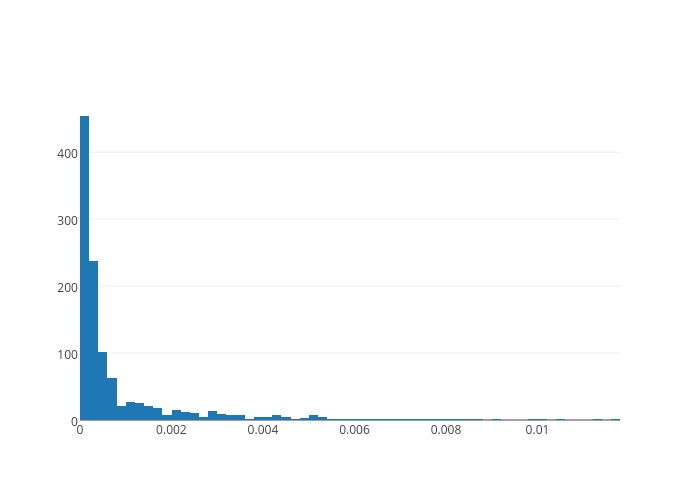
\includegraphics[width=0.28\textwidth]{0am-busy.jpeg}
\end{figure}
This is representative in all (day, hour) combinations. Apparently $p(\alpha, s)$ follows an exponential distribution, where
\begin{align}
p(\alpha, s) = \kappa\frac{L}{s}e^{-\kappa\frac{L}{s}\alpha}
\end{align}
Here $\frac{L}{s}$ is the scale factor for $\kappa$, where $L$ is the constant number of map size. This can be interpreted as the longer distance the driver traveled, the more he/she is likely to see the real distribution. With small value of $s$ (short trip distance), by common sense the driver is more likely to see grids with smaller $\omega$, equivalent to a steeper exponential probability curve after normalization. Now if we substitute $\kappa\frac{L}{s}$ as $\gamma$ into (4), we get 
\begin{align}
\int_{0}^{1}(1-\frac{1}{1+e^{-K(\omega-\mu_\omega)}})\gamma e^{-\gamma\omega}d\omega = \frac{1}{2}
\end{align}
For this equation to hold, we tuned the steepness factor $K$ empirically as $\frac{\mu_\omega}{2\sigma_\omega^2}$. This setup is later proved as work out well.
With the cruise time calculated from $t_c = \frac{v_t}{\alpha v_g}$ and average waiting time $\lambda$, we sample from the process and calculate the pick-up probability:
\begin{align}
p &= \sum_{i=0}^{t_c}\frac{\lambda^ie^{-\lambda}}{i!}
\end{align}
\item Distribution mean, variance. We plot the histogram of trip distance, trip duration, and total pay amount starting from several POI's at different time on Tuesday in figure 2-4.
\begin{figure}
\caption{5pm Little Italy SOHO Trip Time Distribution}
\centering
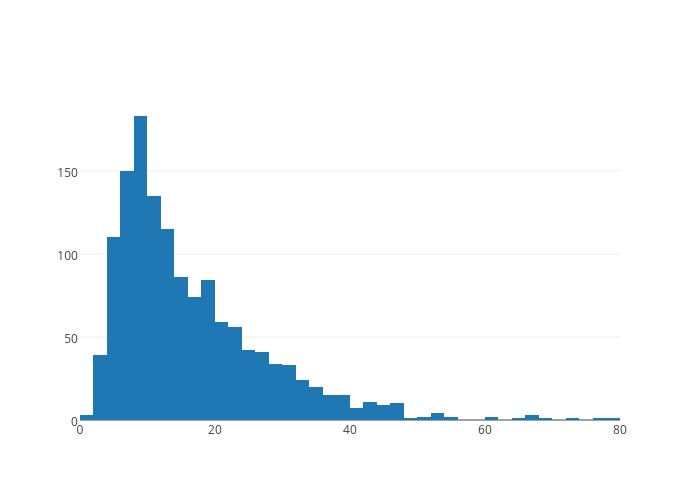
\includegraphics[width=0.28\textwidth]{5pm-littleitaly-soho-triptime.jpeg}
\end{figure}
\begin{figure}
\caption{6pm Lincoln Tunnel Pay Distribution}
\centering
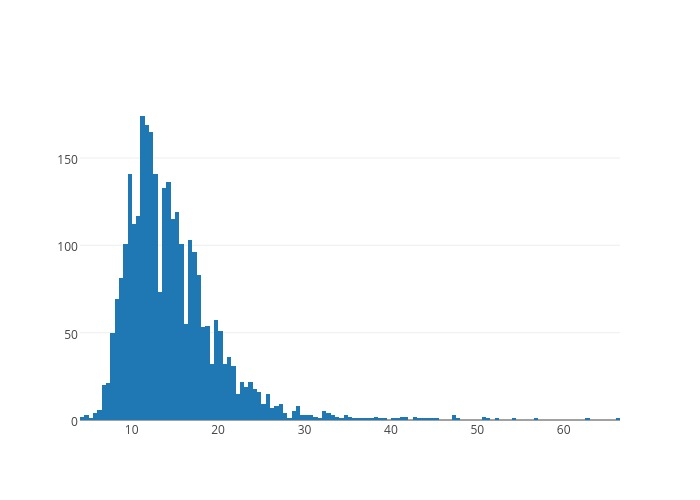
\includegraphics[width=0.28\textwidth]{18-lincoln-tunnel-pay.jpeg}
\end{figure}
\begin{figure}
\caption{11am Sutton Place Trip Distance Distribution}
\centering
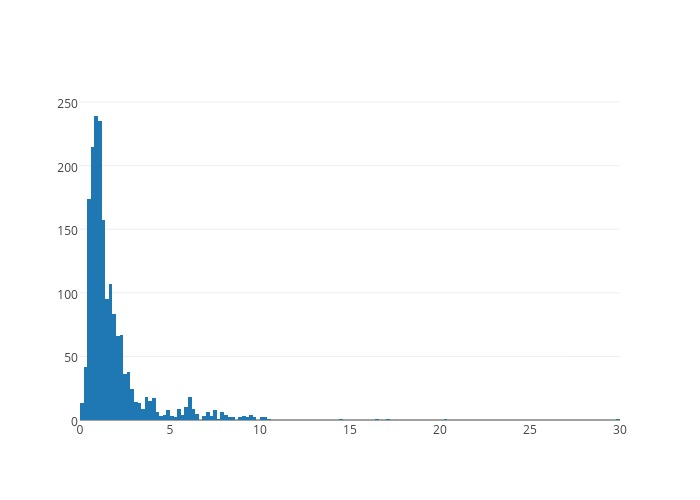
\includegraphics[width=0.28\textwidth]{11am-sutton-place-dist.jpeg}
\end{figure}
Apparently, from the figures, we notice all three distributions are skewed normal. The means and variances of theses distributions are thus effective in evaluating the reward of a grid. Given the numbers, for the specific week day, we define the following reward function for a (grid, hour) key:
\begin{align}
R(g, t) = p\frac{(\mu_p-\frac{\sigma_p}{2})^2}{(\mu_t-\frac{\sigma_t}{2})(\mu_s-\frac{\sigma_s}{2})}
\end{align}
We will discuss later their usage in path simulation. 
\item Drop-off location probability map. This is crucial data for the MDP process and path simulation. Given location-time pair $(g, t)$, we store the mapping 
\begin{align}
\mathcal{M}:(g,t)\to \{(g', \rho_{g'})\}
\end{align}
where $\rho$ is the probability of drop-off at $g'$. Note that $\sum_{g'}\rho_{g'}=1$.
\end{enumerate}
With above parameters described, we visualize a few pick-up probability maps of NYC, generated from a 15-month data set. We also plot the drop-off location map from certain pick-up locations. See figure 5-9.
\begin{figure}
\centering
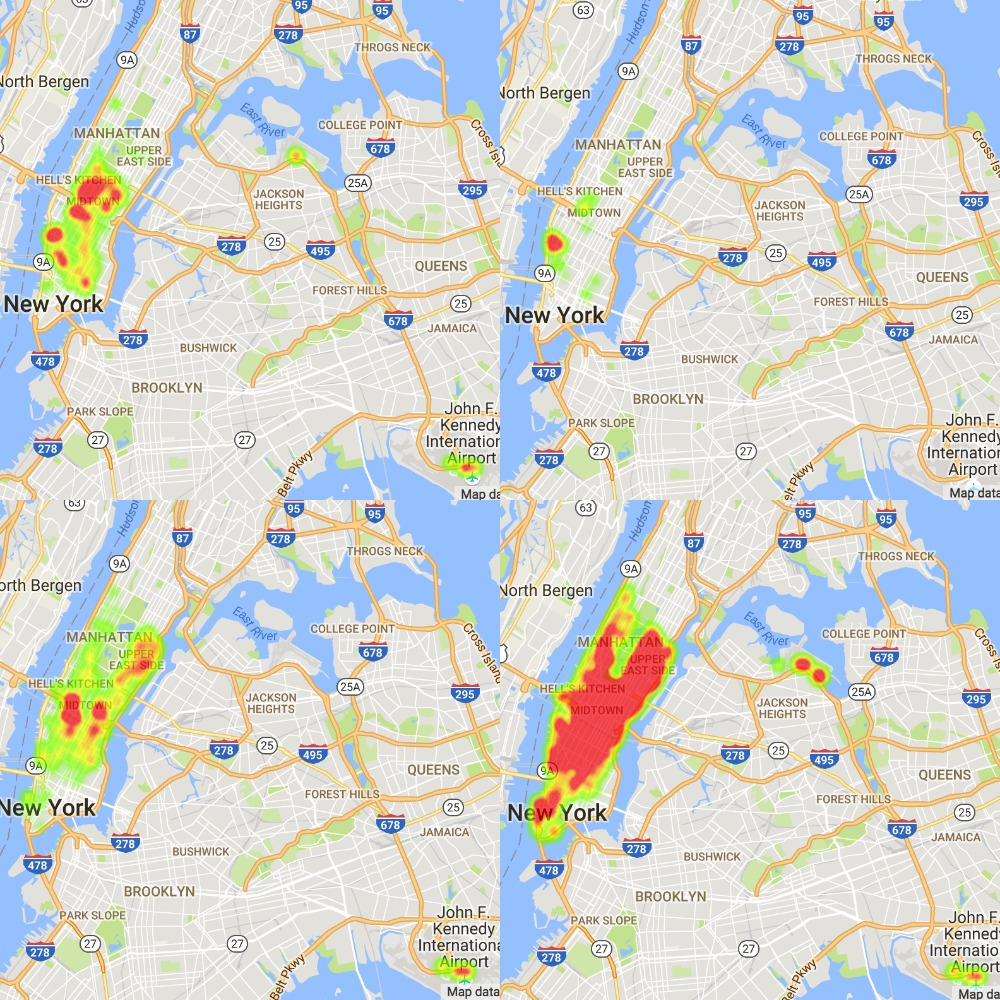
\includegraphics[width=0.3\textwidth]{0-9.jpg}
\caption{From Top-Left to Bottom-Right: 12am, 3am, 6am, 9am}
\end{figure}
\begin{figure}
\centering
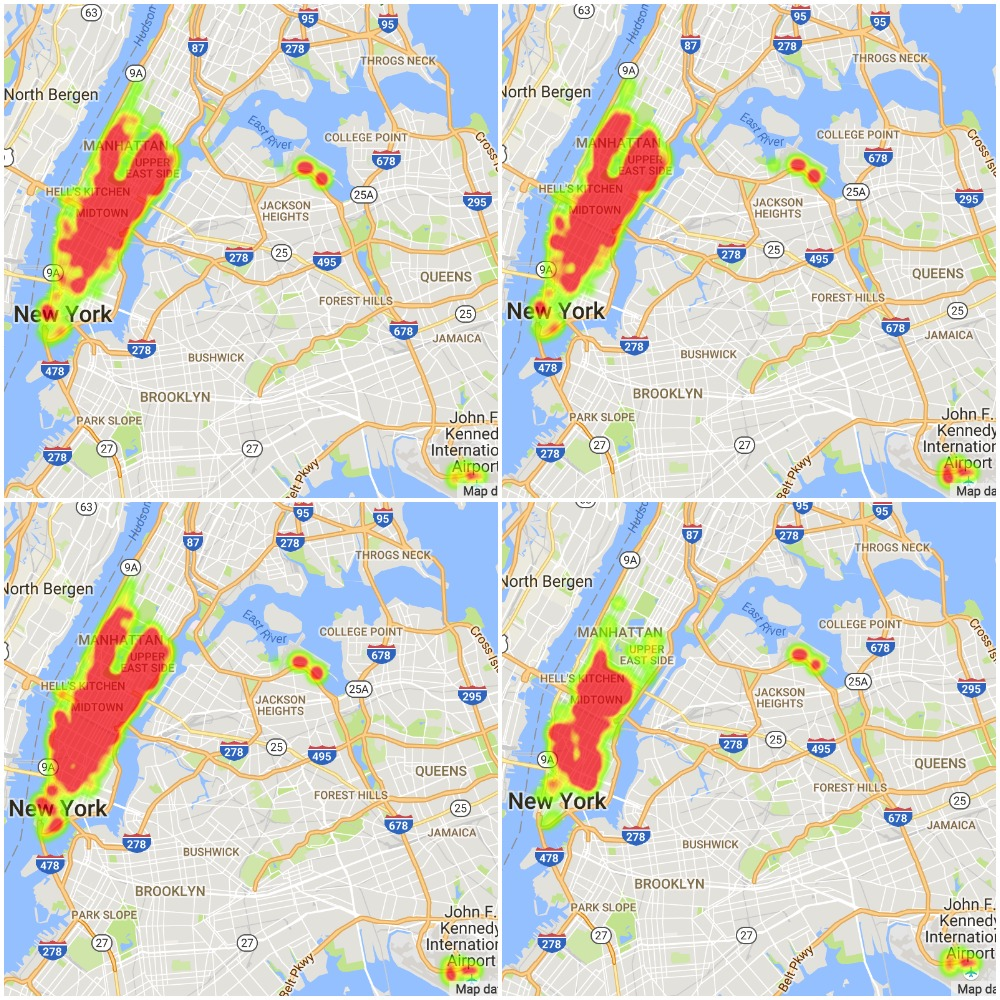
\includegraphics[width=0.3\textwidth]{12-23.jpg}
\caption{From Top-Left to Bottom-Right: 12pm, 15pm, 18pm, 23pm}
\end{figure}
\begin{figure}
\centering
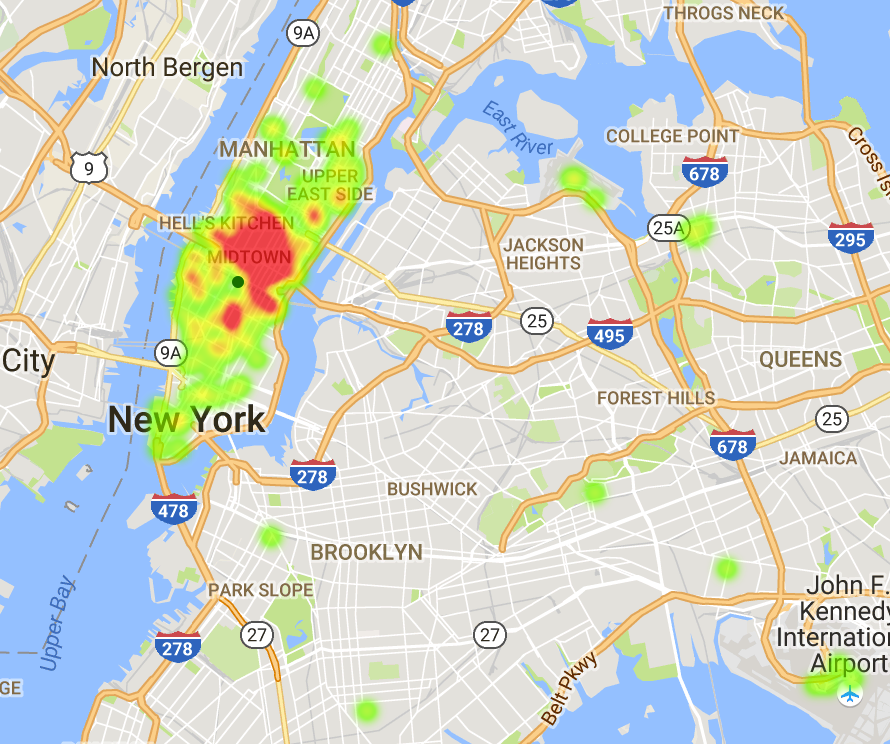
\includegraphics[width=0.33\textwidth]{5pm-empire-state.png}
\caption{5pm Drop-off From Empire State Building}
\end{figure}
\begin{figure}
\centering
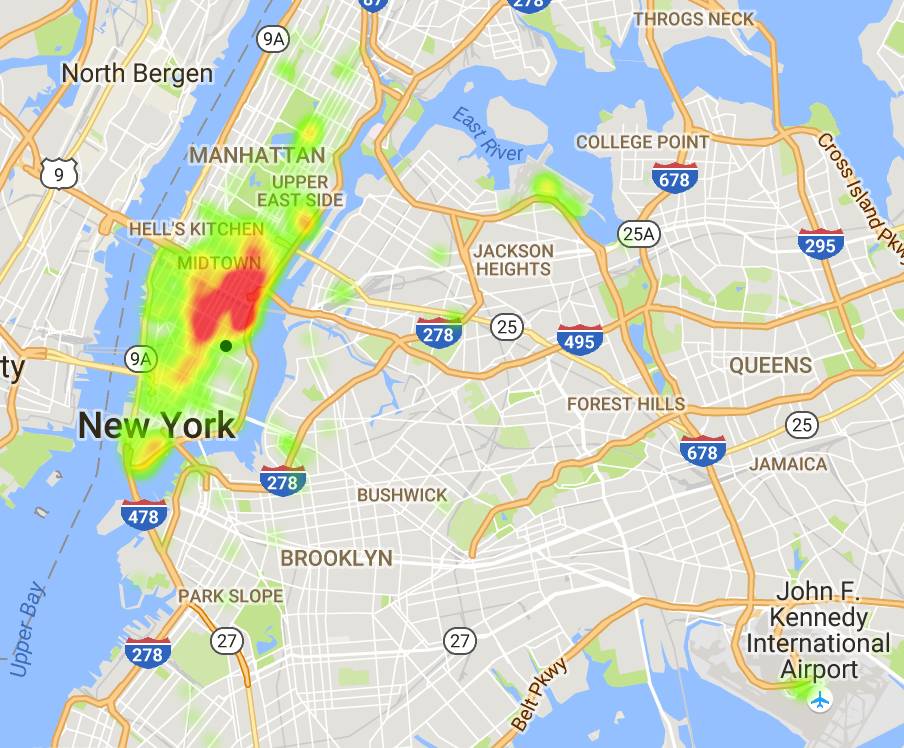
\includegraphics[width=0.33\textwidth]{9-MtSinaiHospital.png}
\caption{9pm Drop-off From Mt. Sinai Hospital}
\end{figure}
\begin{figure}
\centering
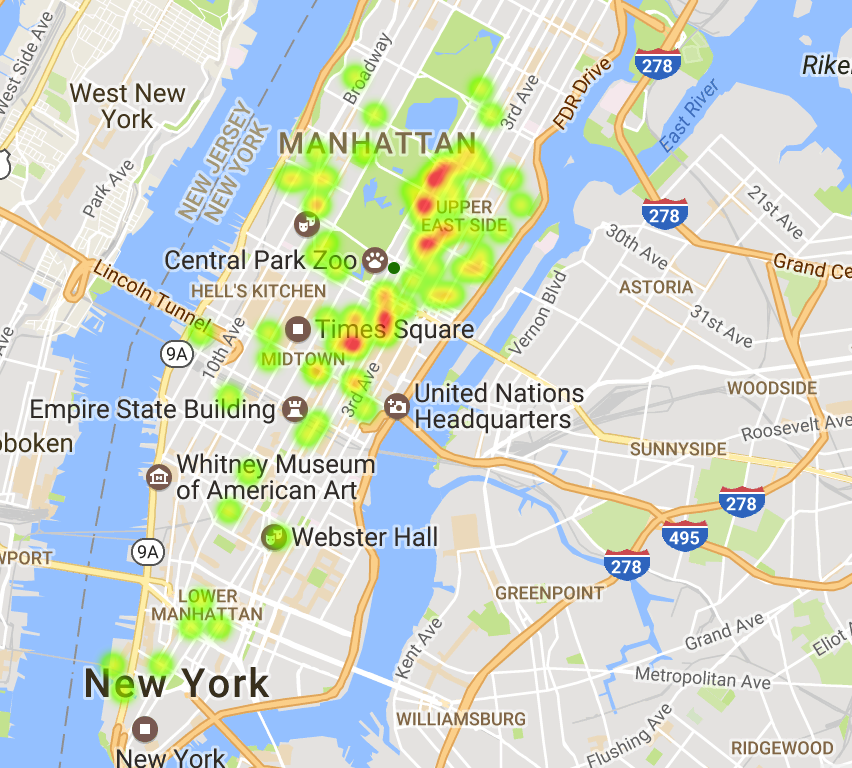
\includegraphics[width=0.33\textwidth]{11-chanel-shop.png}
\caption{11am Drop-off From Chanel Shop}
\end{figure}
\subsection{Markov Decision Process}

\subsection{Policy Generation}
\subsubsection{Learned Policy}

\subsubsection{Baseline Policy}

\subsubsection{Oracle Policy}

\section{Results}
\subsection{Policy Analysis}

\subsection{Visualization of Simulated Path}

\section{Future Works}
\bibliographystyle{ieeetr}
% \bibliography{report}
\end{document}
